% REV00 Tue 04 May 2021 13:55:16 WIB
% START Tue 04 May 2021 13:55:16 WIB

\chapter{XXX}

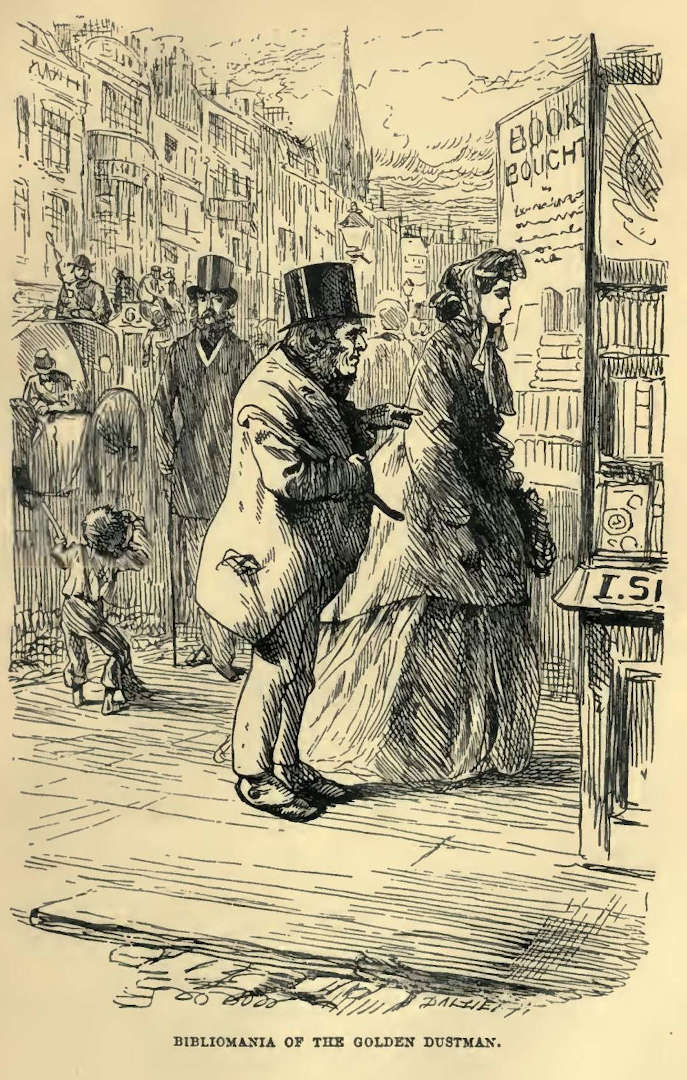
\includegraphics[scale=2.3]{03-05-01}

Chapter 2

THE GOLDEN DUSTMAN RISES A LITTLE


Mr and Mrs Lammle had come to breakfast with Mr and Mrs Boffin. They
were not absolutely uninvited, but had pressed themselves with so much
urgency on the golden couple, that evasion of the honour and pleasure
of their company would have been difficult, if desired. They were in a
charming state of mind, were Mr and Mrs Lammle, and almost as fond of Mr
and Mrs Boffin as of one another.

‘My dear Mrs Boffin,’ said Mrs Lammle, ‘it imparts new life to me, to
see my Alfred in confidential communication with Mr Boffin. The two
were formed to become intimate. So much simplicity combined with so much
force of character, such natural sagacity united to such amiability and
gentleness--these are the distinguishing characteristics of both.’

This being said aloud, gave Mr Lammle an opportunity, as he came with Mr
Boffin from the window to the breakfast table, of taking up his dear and
honoured wife.

‘My Sophronia,’ said that gentleman, ‘your too partial estimate of your
husband’s character--’

‘No! Not too partial, Alfred,’ urged the lady, tenderly moved; ‘never
say that.’

‘My child, your favourable opinion, then, of your husband--you don’t
object to that phrase, darling?’

‘How can I, Alfred?’

‘Your favourable opinion then, my Precious, does less than justice to Mr
Boffin, and more than justice to me.’

‘To the first charge, Alfred, I plead guilty. But to the second, oh no,
no!’

‘Less than justice to Mr Boffin, Sophronia,’ said Mr Lammle, soaring
into a tone of moral grandeur, ‘because it represents Mr Boffin as on my
lower level; more than justice to me, Sophronia, because it represents
me as on Mr Boffin’s higher level. Mr Boffin bears and forbears far more
than I could.’

‘Far more than you could for yourself, Alfred?’

‘My love, that is not the question.’

‘Not the question, Lawyer?’ said Mrs Lammle, archly.

‘No, dear Sophronia. From my lower level, I regard Mr Boffin as too
generous, as possessed of too much clemency, as being too good to
persons who are unworthy of him and ungrateful to him. To those noble
qualities I can lay no claim. On the contrary, they rouse my indignation
when I see them in action.’

‘Alfred!’

‘They rouse my indignation, my dear, against the unworthy persons,
and give me a combative desire to stand between Mr Boffin and all such
persons. Why? Because, in my lower nature I am more worldly and less
delicate. Not being so magnanimous as Mr Boffin, I feel his injuries
more than he does himself, and feel more capable of opposing his
injurers.’

It struck Mrs Lammle that it appeared rather difficult this morning
to bring Mr and Mrs Boffin into agreeable conversation. Here had been
several lures thrown out, and neither of them had uttered a word. Here
were she, Mrs Lammle, and her husband discoursing at once affectingly
and effectively, but discoursing alone. Assuming that the dear old
creatures were impressed by what they heard, still one would like to be
sure of it, the more so, as at least one of the dear old creatures
was somewhat pointedly referred to. If the dear old creatures were too
bashful or too dull to assume their required places in the discussion,
why then it would seem desirable that the dear old creatures should be
taken by their heads and shoulders and brought into it.

‘But is not my husband saying in effect,’ asked Mrs Lammle, therefore,
with an innocent air, of Mr and Mrs Boffin, ‘that he becomes unmindful
of his own temporary misfortunes in his admiration of another whom he is
burning to serve? And is not that making an admission that his nature is
a generous one? I am wretched in argument, but surely this is so, dear
Mr and Mrs Boffin?’

Still, neither Mr and Mrs Boffin said a word. He sat with his eyes on
his plate, eating his muffins and ham, and she sat shyly looking at the
teapot. Mrs Lammle’s innocent appeal was merely thrown into the air, to
mingle with the steam of the urn. Glancing towards Mr and Mrs Boffin,
she very slightly raised her eyebrows, as though inquiring of her
husband: ‘Do I notice anything wrong here?’

Mr Lammle, who had found his chest effective on a variety of occasions,
manoeuvred his capacious shirt front into the largest demonstration
possible, and then smiling retorted on his wife, thus:

‘Sophronia, darling, Mr and Mrs Boffin will remind you of the old adage,
that self-praise is no recommendation.’

‘Self-praise, Alfred? Do you mean because we are one and the same?’

‘No, my dear child. I mean that you cannot fail to remember, if you
reflect for a single moment, that what you are pleased to compliment me
upon feeling in the case of Mr Boffin, you have yourself confided to me
as your own feeling in the case of Mrs Boffin.’

[‘I shall be beaten by this Lawyer,’ Mrs Lammle gaily whispered to
Mrs Boffin. ‘I am afraid I must admit it, if he presses me, for it’s
damagingly true.’)

Several white dints began to come and go about Mr Lammle’s nose, as he
observed that Mrs Boffin merely looked up from the teapot for a moment
with an embarrassed smile, which was no smile, and then looked down
again.

‘Do you admit the charge, Sophronia?’ inquired Alfred, in a rallying
tone.

‘Really, I think,’ said Mrs Lammle, still gaily, ‘I must throw myself
on the protection of the Court. Am I bound to answer that question, my
Lord?’ To Mr Boffin.

‘You needn’t, if you don’t like, ma’am,’ was his answer. ‘It’s not of
the least consequence.’

Both husband and wife glanced at him, very doubtfully. His manner was
grave, but not coarse, and derived some dignity from a certain repressed
dislike of the tone of the conversation.

Again Mrs Lammle raised her eyebrows for instruction from her husband.
He replied in a slight nod, ‘Try ‘em again.’

‘To protect myself against the suspicion of covert self-laudation, my
dear Mrs Boffin,’ said the airy Mrs Lammle therefore, ‘I must tell you
how it was.’

‘No. Pray don’t,’ Mr Boffin interposed.

Mrs Lammle turned to him laughingly. ‘The Court objects?’

‘Ma’am,’ said Mr Boffin, ‘the Court (if I am the Court) does object. The
Court objects for two reasons. First, because the Court don’t think it
fair. Secondly, because the dear old lady, Mrs Court (if I am Mr) gets
distressed by it.’

A very remarkable wavering between two bearings--between her
propitiatory bearing there, and her defiant bearing at Mr Twemlow’s--was
observable on the part of Mrs Lammle as she said:

‘What does the Court not consider fair?’

‘Letting you go on,’ replied Mr Boffin, nodding his head soothingly, as
who should say, We won’t be harder on you than we can help; we’ll make
the best of it. ‘It’s not above-board and it’s not fair. When the old
lady is uncomfortable, there’s sure to be good reason for it. I see she
is uncomfortable, and I plainly see this is the good reason wherefore.
HAVE you breakfasted, ma’am.’

Mrs Lammle, settling into her defiant manner, pushed her plate away,
looked at her husband, and laughed; but by no means gaily.

‘Have YOU breakfasted, sir?’ inquired Mr Boffin.

‘Thank you,’ replied Alfred, showing all his teeth. ‘If Mrs Boffin will
oblige me, I’ll take another cup of tea.’

He spilled a little of it over the chest which ought to have been so
effective, and which had done so little; but on the whole drank it with
something of an air, though the coming and going dints got almost as
large, the while, as if they had been made by pressure of the teaspoon.
‘A thousand thanks,’ he then observed. ‘I have breakfasted.’

‘Now, which,’ said Mr Boffin softly, taking out a pocket-book, ‘which of
you two is Cashier?’

‘Sophronia, my dear,’ remarked her husband, as he leaned back in his
chair, waving his right hand towards her, while he hung his left hand
by the thumb in the arm-hole of his waistcoat: ‘it shall be your
department.’

‘I would rather,’ said Mr Boffin, ‘that it was your husband’s, ma’am,
because--but never mind, because, I would rather have to do with him.
However, what I have to say, I will say with as little offence as
possible; if I can say it without any, I shall be heartily glad. You two
have done me a service, a very great service, in doing what you did (my
old lady knows what it was), and I have put into this envelope a bank
note for a hundred pound. I consider the service well worth a hundred
pound, and I am well pleased to pay the money. Would you do me the
favour to take it, and likewise to accept my thanks?’

With a haughty action, and without looking towards him, Mrs Lammle held
out her left hand, and into it Mr Boffin put the little packet. When she
had conveyed it to her bosom, Mr Lammle had the appearance of feeling
relieved, and breathing more freely, as not having been quite certain
that the hundred pounds were his, until the note had been safely
transferred out of Mr Boffin’s keeping into his own Sophronia’s.

‘It is not impossible,’ said Mr Boffin, addressing Alfred, ‘that you
have had some general idea, sir, of replacing Rokesmith, in course of
time?’

‘It is not,’ assented Alfred, with a glittering smile and a great deal
of nose, ‘not impossible.’

‘And perhaps, ma’am,’ pursued Mr Boffin, addressing Sophronia, ‘you have
been so kind as to take up my old lady in your own mind, and to do her
the honour of turning the question over whether you mightn’t one of
these days have her in charge, like? Whether you mightn’t be a sort of
Miss Bella Wilfer to her, and something more?’

‘I should hope,’ returned Mrs Lammle, with a scornful look and in a loud
voice, ‘that if I were anything to your wife, sir, I could hardly fail
to be something more than Miss Bella Wilfer, as you call her.’

‘What do YOU call her, ma’am?’ asked Mr Boffin.

Mrs Lammle disdained to reply, and sat defiantly beating one foot on the
ground.

‘Again I think I may say, that’s not impossible. Is it, sir?’ asked Mr
Boffin, turning to Alfred.

‘It is not,’ said Alfred, smiling assent as before, ‘not impossible.’

‘Now,’ said Mr Boffin, gently, ‘it won’t do. I don’t wish to say a
single word that might be afterwards remembered as unpleasant; but it
won’t do.’

‘Sophronia, my love,’ her husband repeated in a bantering manner, ‘you
hear? It won’t do.’

‘No,’ said Mr Boffin, with his voice still dropped, ‘it really won’t.
You positively must excuse us. If you’ll go your way, we’ll go ours, and
so I hope this affair ends to the satisfaction of all parties.’

Mrs Lammle gave him the look of a decidedly dissatisfied party demanding
exemption from the category; but said nothing.

‘The best thing we can make of the affair,’ said Mr Boffin, ‘is a matter
of business, and as a matter of business it’s brought to a conclusion.
You have done me a great service, a very great service, and I have paid
for it. Is there any objection to the price?’

Mr and Mrs Lammle looked at one another across the table, but neither
could say that there was. Mr Lammle shrugged his shoulders, and Mrs
Lammle sat rigid.

‘Very good,’ said Mr Boffin. ‘We hope (my old lady and me) that you’ll
give us credit for taking the plainest and honestest short-cut that
could be taken under the circumstances. We have talked it over with a
deal of care (my old lady and me), and we have felt that at all to lead
you on, or even at all to let you go on of your own selves, wouldn’t be
the right thing. So, I have openly given you to understand that--’
Mr Boffin sought for a new turn of speech, but could find none so
expressive as his former one, repeated in a confidential tone, ‘--that
it won’t do. If I could have put the case more pleasantly I would; but
I hope I haven’t put it very unpleasantly; at all events I haven’t meant
to. So,’ said Mr Boffin, by way of peroration, ‘wishing you well in the
way you go, we now conclude with the observation that perhaps you’ll go
it.’

Mr Lammle rose with an impudent laugh on his side of the table, and Mrs
Lammle rose with a disdainful frown on hers. At this moment a hasty foot
was heard on the staircase, and Georgiana Podsnap broke into the room,
unannounced and in tears.

‘Oh, my dear Sophronia,’ cried Georgiana, wringing her hands as she ran
up to embrace her, ‘to think that you and Alfred should be ruined! Oh,
my poor dear Sophronia, to think that you should have had a Sale at your
house after all your kindness to me! Oh, Mr and Mrs Boffin, pray forgive
me for this intrusion, but you don’t know how fond I was of Sophronia
when Pa wouldn’t let me go there any more, or what I have felt for
Sophronia since I heard from Ma of her having been brought low in the
world. You don’t, you can’t, you never can, think, how I have lain awake
at night and cried for my good Sophronia, my first and only friend!’

Mrs Lammle’s manner changed under the poor silly girl’s embraces, and
she turned extremely pale: directing one appealing look, first to Mrs
Boffin, and then to Mr Boffin. Both understood her instantly, with
a more delicate subtlety than much better educated people, whose
perception came less directly from the heart, could have brought to bear
upon the case.

‘I haven’t a minute,’ said poor little Georgiana, ‘to stay. I am out
shopping early with Ma, and I said I had a headache and got Ma to leave
me outside in the phaeton, in Piccadilly, and ran round to Sackville
Street, and heard that Sophronia was here, and then Ma came to see, oh
such a dreadful old stony woman from the country in a turban in Portland
Place, and I said I wouldn’t go up with Ma but would drive round and
leave cards for the Boffins, which is taking a liberty with the name;
but oh my goodness I am distracted, and the phaeton’s at the door, and
what would Pa say if he knew it!’

‘Don’t ye be timid, my dear,’ said Mrs Boffin. ‘You came in to see us.’

‘Oh, no, I didn’t,’ cried Georgiana. ‘It’s very impolite, I know, but
I came to see my poor Sophronia, my only friend. Oh! how I felt the
separation, my dear Sophronia, before I knew you were brought low in the
world, and how much more I feel it now!’

There were actually tears in the bold woman’s eyes, as the soft-headed
and soft-hearted girl twined her arms about her neck.

‘But I’ve come on business,’ said Georgiana, sobbing and drying her
face, and then searching in a little reticule, ‘and if I don’t despatch
it I shall have come for nothing, and oh good gracious! what would Pa
say if he knew of Sackville Street, and what would Ma say if she was
kept waiting on the doorsteps of that dreadful turban, and there never
were such pawing horses as ours unsettling my mind every moment more
and more when I want more mind than I have got, by pawing up Mr Boffin’s
street where they have no business to be. Oh! where is, where is it?
Oh! I can’t find it!’ All this time sobbing, and searching in the little
reticule.

‘What do you miss, my dear?’ asked Mr Boffin, stepping forward.

‘Oh! it’s little enough,’ replied Georgiana, ‘because Ma always treats
me as if I was in the nursery (I am sure I wish I was!), but I hardly
ever spend it and it has mounted up to fifteen pounds, Sophronia, and I
hope three five-pound notes are better than nothing, though so little,
so little! And now I have found that--oh, my goodness! there’s the other
gone next! Oh no, it isn’t, here it is!’

With that, always sobbing and searching in the reticule, Georgiana
produced a necklace.

‘Ma says chits and jewels have no business together,’ pursued Georgiana,
‘and that’s the reason why I have no trinkets except this, but I suppose
my aunt Hawkinson was of a different opinion, because she left me this,
though I used to think she might just as well have buried it, for it’s
always kept in jewellers’ cotton. However, here it is, I am thankful
to say, and of use at last, and you’ll sell it, dear Sophronia, and buy
things with it.’

‘Give it to me,’ said Mr Boffin, gently taking it. ‘I’ll see that it’s
properly disposed of.’

‘Oh! are you such a friend of Sophronia’s, Mr Boffin?’ cried Georgiana.
‘Oh, how good of you! Oh, my gracious! there was something else, and
it’s gone out of my head! Oh no, it isn’t, I remember what it was. My
grandmamma’s property, that’ll come to me when I am of age, Mr Boffin,
will be all my own, and neither Pa nor Ma nor anybody else will have
any control over it, and what I wish to do it so make some of it over
somehow to Sophronia and Alfred, by signing something somewhere that’ll
prevail on somebody to advance them something. I want them to have
something handsome to bring them up in the world again. Oh, my goodness
me! Being such a friend of my dear Sophronia’s, you won’t refuse me,
will you?’

‘No, no,’ said Mr Boffin, ‘it shall be seen to.’

‘Oh, thank you, thank you!’ cried Georgiana. ‘If my maid had a little
note and half a crown, I could run round to the pastrycook’s to sign
something, or I could sign something in the Square if somebody would
come and cough for me to let ‘em in with the key, and would bring a pen
and ink with ‘em and a bit of blotting-paper. Oh, my gracious! I must
tear myself away, or Pa and Ma will both find out! Dear, dear Sophronia,
good, good-bye!’

The credulous little creature again embraced Mrs Lammle most
affectionately, and then held out her hand to Mr Lammle.

‘Good-bye, dear Mr Lammle--I mean Alfred. You won’t think after to-day
that I have deserted you and Sophronia because you have been brought low
in the world, will you? Oh me! oh me! I have been crying my eyes out of
my head, and Ma will be sure to ask me what’s the matter. Oh, take me
down, somebody, please, please, please!’

Mr Boffin took her down, and saw her driven away, with her poor
little red eyes and weak chin peering over the great apron of the
custard-coloured phaeton, as if she had been ordered to expiate some
childish misdemeanour by going to bed in the daylight, and were peeping
over the counterpane in a miserable flutter of repentance and low
spirits. Returning to the breakfast-room, he found Mrs Lammle still
standing on her side of the table, and Mr Lammle on his.

‘I’ll take care,’ said Mr Boffin, showing the money and the necklace,
‘that these are soon given back.’

Mrs Lammle had taken up her parasol from a side table, and stood
sketching with it on the pattern of the damask cloth, as she had
sketched on the pattern of Mr Twemlow’s papered wall.

‘You will not undeceive her I hope, Mr Boffin?’ she said, turning her
head towards him, but not her eyes.

‘No,’ said Mr Boffin.

‘I mean, as to the worth and value of her friend,’ Mrs Lammle explained,
in a measured voice, and with an emphasis on her last word.

‘No,’ he returned. ‘I may try to give a hint at her home that she is in
want of kind and careful protection, but I shall say no more than that
to her parents, and I shall say nothing to the young lady herself.’

‘Mr and Mrs Boffin,’ said Mrs Lammle, still sketching, and seeming to
bestow great pains upon it, ‘there are not many people, I think, who,
under the circumstances, would have been so considerate and sparing as
you have been to me just now. Do you care to be thanked?’

‘Thanks are always worth having,’ said Mrs Boffin, in her ready good
nature.

‘Then thank you both.’

‘Sophronia,’ asked her husband, mockingly, ‘are you sentimental?’

‘Well, well, my good sir,’ Mr Boffin interposed, ‘it’s a very good
thing to think well of another person, and it’s a very good thing to be
thought well of BY another person. Mrs Lammle will be none the worse for
it, if she is.’

‘Much obliged. But I asked Mrs Lammle if she was.’

She stood sketching on the table-cloth, with her face clouded and set,
and was silent.

‘Because,’ said Alfred, ‘I am disposed to be sentimental myself, on
your appropriation of the jewels and the money, Mr Boffin. As our little
Georgiana said, three five-pound notes are better than nothing, and if
you sell a necklace you can buy things with the produce.’

‘IF you sell it,’ was Mr Boffin’s comment, as he put it in his pocket.

Alfred followed it with his looks, and also greedily pursued the notes
until they vanished into Mr Boffin’s waistcoat pocket. Then he directed
a look, half exasperated and half jeering, at his wife. She still stood
sketching; but, as she sketched, there was a struggle within her, which
found expression in the depth of the few last lines the parasol point
indented into the table-cloth, and then some tears fell from her eyes.

‘Why, confound the woman,’ exclaimed Lammle, ‘she IS sentimental!

She walked to the window, flinching under his angry stare, looked out
for a moment, and turned round quite coldly.

‘You have had no former cause of complaint on the sentimental score,
Alfred, and you will have none in future. It is not worth your noticing.
We go abroad soon, with the money we have earned here?’

‘You know we do; you know we must.’

‘There is no fear of my taking any sentiment with me. I should soon be
eased of it, if I did. But it will be all left behind. It IS all left
behind. Are you ready, Alfred?’

‘What the deuce have I been waiting for but you, Sophronia?’

‘Let us go then. I am sorry I have delayed our dignified departure.’

She passed out and he followed her. Mr and Mrs Boffin had the curiosity
softly to raise a window and look after them as they went down the long
street. They walked arm-in-arm, showily enough, but without appearing
to interchange a syllable. It might have been fanciful to suppose that
under their outer bearing there was something of the shamed air of two
cheats who were linked together by concealed handcuffs; but, not so, to
suppose that they were haggardly weary of one another, of themselves,
and of all this world. In turning the street corner they might have
turned out of this world, for anything Mr and Mrs Boffin ever saw of
them to the contrary; for, they set eyes on the Lammles never more.



